\documentclass[dvips, a4paper, listsleft, 12pt, openany, oneside]{scrbook}
% new koma package
\usepackage{scrpage2}

\usepackage{ae}
\usepackage[latin1]{inputenc}
\usepackage[ngerman]{babel}
\usepackage{listings}
%\usepackage[isolatin]{inputenc}
\usepackage[T1]{fontenc}
\usepackage{verbatim}
% \usepackage[small]{caption2}
\usepackage[]{graphicx,psfrag}
\DeclareGraphicsExtensions{.png,.PNG,.pdf,.eps,.bmp}
\usepackage{amsmath}
\usepackage{amsfonts}
\usepackage{amssymb}
\usepackage[dvips]{color}
\usepackage{xspace}
\usepackage{bm}
% \usepackage{bbm}
% \usepackage{slashbox}
\usepackage{booktabs} % extends the tables property by: \toprule, \midrule and \bottomrule
\usepackage{longtable}
\usepackage{array}


%%%%%%%%%%%%%%%%%%%%%%%%%%%%%%%%%%%%%%%%%%%%%%%%%%%%%%%%%%%%
% if hyperrefs are desired, uncomment the appropriate lines in the following block;

% define your own link color(including: \cite, \ref, \eqref, \footnote, ...)
% \definecolor{darkblue}{rgb}{0,0,.62} 
% or:
% \definecolor{darkblue}{rgb}{0,.19,.40}

% \usepackage[breaklinks, colorlinks, urlcolor=darkblue]{hyperref}
% \usepackage{hypcap}
% NOTE: sometimes problems arise when using hyperref;
%       especially the dvi/ps file might look different from what you expected;
\usepackage{url}

%%%%%%%%%%%%%%%%%%%%%%%%%%%%%%%%%%%%%%%%%%%%%%%%%%%%%%%%%%%%
% for koma headers
\pagestyle{scrheadings}
% define head and foot marks
\renewcommand{\chaptermark}[1]{\markboth{#1}{}}
\renewcommand{\sectionmark}[1]{\markright{-~#1}{}}
\ihead{\leftmark}
\chead{}
\ohead{\pagemark}
\cfoot{}
\setheadsepline{.4pt}

%%%%%%%%%%%%%%%%%%%%%%%%%%%%%%%%%%%%%%%%%%%%%%%%%%%%%%%%%%%%
% chapter head change
% adding lines above the chapter head
% 1st get a new command
\newcommand*{\ORIGchapterheadstartvskip}{}%
% 2nd save the original definition to the new command
\let\ORIGchapterheadstartvskip=\chapterheadstartvskip
% 3rd redefine the command using the saved original command
\renewcommand*{\chapterheadstartvskip}{%
  \ORIGchapterheadstartvskip
  {%
    \setlength{\parskip}{0pt}%
    \noindent\rule[0.3\baselineskip]{\linewidth}{0.8pt}\par
  }%
}
% and below the chapter head
\newcommand*{\ORIGchapterheadendvskip}{}%
\let\ORIGchapterheadendvskip=\chapterheadendvskip
\renewcommand*{\chapterheadendvskip}{%
  {%
    \setlength{\parskip}{0pt}%
    \noindent\rule[0.3\baselineskip]{\linewidth}{0.8pt}\par
  }%
  \ORIGchapterheadendvskip
}

% %%%%%%%%%%%%%%%%%%%%%%%%%%%%%%%%%%%%%%%%%%%%%%%%%%%%%%%%%%%%
% % list of abbreviations
% \usepackage{nomencl}
% % rename command to 'abk'
% \let\abk\nomenclature
% % title in german
% \renewcommand{\nomname}{Abk�rzungsverzeichnis}
% % define space between abbreviation and declaration
% \setlength{\nomlabelwidth}{.25\hsize}
% \renewcommand{\nomlabel}[1]{#1 \dotfill}
% % decrease row spacing
% \setlength{\nomitemsep}{-\parsep}
% \makeglossary
% % new command: highlighting abbrevation letters in declaration part
% \usepackage[normalem]{ulem}
% \newcommand{\markup}[1]{\textbf{#1}}
% 
% %%%%%%%%%%%%%%%%%%%%%%%%%%%%%%%%%%%%%%%%%%%%%%%%%%%%%%%%%%%%
% % define german names
%   \def\prefacename{Vorwort}%
%   \def\refname{Literatur}%
%   \def\abstractname{Zusammenfassung}%
%   \def\bibname{Literaturverzeichnis}%
%   \def\chaptername{Kapitel}%
%   \def\appendixname{Anhang}%
%   \def\contentsname{Inhaltsverzeichnis}% % oder nur: Inhalt
%   \def\listfigurename{Abbildungsverzeichnis}%
%   \def\listtablename{Tabellenverzeichnis}%
%   \def\indexname{Index}%
%   \def\figurename{Abbildung}%
%   \def\tablename{Tabelle}%  % or: Tafel
%   \def\partname{Teil}%
%   \def\enclname{Anlage(n)}% % or: Beilage(n)
%   \def\ccname{Verteiler}%   % or: Kopien an
%   \def\headtoname{An}%
%   \def\pagename{Seite}%
%   \def\seename{siehe}%
%   \def\alsoname{siehe auch}

%%%%%%%%%%%%%%%%%%%%%%%%%%%%%%%%%%%%%%%%%%%%%%%%%%%%%%%%%%%%
% define pagesize
\setlength{\oddsidemargin}{5mm}
\setlength{\evensidemargin}{5mm}
\setlength{\textwidth}{155mm}
\setlength{\topmargin}{-5mm}
\setlength{\textheight}{235mm}

%%%%%%%%%%%%%%%%%%%%%%%%%%%%%%%%%%%%%%%%%%%%%%%%%%%%%%%%%%%%
% special formatted strings
\newcommand{\matlab}{\emph{MATLAB}\xspace}
\newcommand{\intel}{\emph{INTEL}\xspace}

%%%%%%%%%%%%%%%%%%%%%%%%%%%%%%%%%%%%%%%%%%%%%%%%%%%%%%%%%%%%
% changing some fonts 
% \renewcommand{\captionlabelfont}{\small\sffamily\bfseries}
% \setcaphanging
% 
% \setkomafont{pagehead}{%
% \normalfont\sffamily\bfseries
% }
% \setkomafont{pagenumber}{%
% \normalfont\rmfamily\slshape
% }

%%%%%%%%%%%%%%%%%%%%%%%%%%%%%%%%%%%%%%%%%%%%%%%%%%%%%%%%%%%%
% command for the list of symbols
\newcommand{\listsymbol}[2]{#1$\;\;$\dotfill$\;\;$&#2\\}

% define graficspath

\graphicspath{{bilder/}{bilder/Kapitel_1/}{bilder/Kapitel_2/}}
\begin{document}
%%%%%%%%%%%%%%%%%%%%
% the customized title page
% this is the title page 
\begin{titlepage}
\begin{center}
  \begin{figure}
    \begin{center}
      
\includegraphics[scale=0.5]{bilder/uni_logo.eps}
    \end{center}
  \end{figure}
\normalsize{\textbf{Institut f�r Elektrotechnik und Informationstechnik}\\
Universit�t Paderborn\\
Fachgebiet Nachrichtentechnik\\
Prof. Dr.-Ing. Reinhold H�b-Umbach\\}
\vfill {\bf {\Large Seminararbeit} \linebreak \\ \LARGE{Training des statistischen Sprachmodells}}
\renewcommand{\baselinestretch}{2}\normalsize
\vfill{von\\ {\large Buyu Xiao\\ Matr.-Nr.: 6436310}}
\renewcommand{\baselinestretch}{1,5}\normalsize
\vfill{
  \begin{flushleft}
    Betreuer: Volker Leutnant\\
  \end{flushleft}
}
\renewcommand{\baselinestretch}{1}\normalsize
\end{center}
\end{titlepage}
% 
% %%%%%%%%%%%%%%%%%%%%
% % frontmatter
% \frontmatter
% \tableofcontents
% \clearpage
% % list of figures
% \addcontentsline{toc}{chapter}{Abbildungsverzeichnis}
% \listoffigures
% \clearpage
% % list of tables
% \addcontentsline{toc}{chapter}{Tabellenverzeichnis}
% \listoftables
% \clearpage
% %list of equation symbols 
% \include{symbols}
% \clearpage
% % list of abbreviations
% \addcontentsline{toc}{chapter}{Abk�rzungsverzeichnis}
% % \printglossary
% \clearpage
% \newpage
% \mbox{} \thispagestyle{empty} \newpage

%%%%%%%%%%%%%%%%%%%%
% mainmatter
\mainmatter
% make the header to include the chapter numbering
% from now on
\ihead{\thechapter~\leftmark} %~\rightmark}

%inhalt_main
\chapter{Einleitung}
\label{chapter:Einleitung}
%\section{Einleitung}
	%Einleitung
Bei einem Spracherkkenner ist die Sprachmodellierung sehr schwer. Um ein Sprachmodell f\"ur eine bestimmte Sprache zu entwerfen, muss man aus dem Trainingskorpus die Bedingung Wahrscheinlichkeit $p(w_{n}|w_{1},..w_{n-1})$   vom Sprachmodell $p(w_{1}^n)$   bestimmen.

Die vorliegende Hausarbeit versucht zu erkl\"aren, wie ein realisierbares Modell durch Training erzeugt wird und die L\"osung des Problems bei den eingeschr\"ankten Trainingdatenbasen erreicht wird. 

Um diese zu erreichen, werden in diesem Artikel zuerst ein approximatives Modell, M-Gramm, und unterschiedliche Discounting-Algorithmuen f\"ur das 0-Wahrscheinlichkeitsproblem vorgestellt. Am Ende werden unsere Ergebnisse durch ein SLM-Toolkit angezeigt.

	
\chapter{Statisches Sprachmodell}
\label{chapter:Sprach-Modell}

\section{Statisches Sprachmodell}
	%Statische Sprach_Modell

Was ist ein statisches Sprachmodell? Ein statische Sprachmodell wird durch die Wahrscheinlichkeit $p(w_{1}^n)$ von Wortfolgen  dargestellt.
Im folgenden Anwendungsbereich[1] spielt das Sprachmodell eine grosse Rolle.
\begin{itemize}
	\item Vereinfachen eines Spracherkenners
	\item Text-Komprimierung
	\item Extraktion von Schl\"usselw\"ortern aus Texten
	\item etc...
\end{itemize}
Im Detail, extrahiert das Sprachmodell die Eigenschaft, das Schlusswort oder die Syntax aus der Sprache.\footnote{Eine Sprache hat riesiggro\ss en Wortschatz und unendliche M\"oglichkeiten der Wortfolgen. D.h. ein Spracherkenner soll unendliche Wortfolgen kennen. Aber eine Sprache ist immer regul\"ar. Durch das Sprachmodell muss ein Spracherkenner  nur  limitierte Regeln speichern.}
Bei der Text-Komprimierung speichert man nur einmal die im Text immer wieder auftretenden W\"orter. Ein bekanntes Beispiel bei der Extraktion von Schl\"usselw\"orter ist das Tippprogramm. Man gibt erst Buchstaben ein und das Programm zeigt die m\"oglichen \"ubrigen Teile.

	\subsection{M-Gramm}
  	%M_Gramm
Eine ideale Darstellung des statistischen Sprachmodells ist wie die Gleichung (2.1), die die Wahrscheinlichkeit einer Wortkette bezeichnet. Um die Wahrscheinlichkeit $p(w_{1}^n)$ zu bestimmt m\"ussen die auftretende Wahrscheinlichkeit des Wortes $w_{1}$ und die bedingte Wahrscheinlichkeit f\"ur $w_{2}...w_{n}$ bekannt sein.
\\
\\
\begin{align}
p(w_{1}^n) = p(w_{1},w_{2}...w_{n}) &= \prod_{i=1}^n p(w_{i}|w_{1},..w_{i-1}) \nonumber\\
&= p(w_{1})p(w_{2}|w_{1})...p(w_{n}|w_{1},..w_{n-1})
\end{align}
\\
\\
\cite{book_speech} erkl\"art , dass die Wortkettenl\"ange n theoretisch unendlich gro\ss  sein kann und die Wahrscheinlichkeit $p(w_{n}|w_{1}^n)$ nicht berechenbar wird. Man geht auf eine Approximation der bedingten Wahrscheinlichkeit ein durch Beschr\"ankung der "`History"' in der Bedingung. Die genaue Idee ist, dass man alle bedingten Wahrscheinlichkeiten $p(w_{n}|w_{1}...w_{n})$, f\"ur die die letzten m-1 Vorg\"angerw\"orter von $w_{n}$ identisch sind, zu einer \"Aquivalenzklasse zusammenfasst. Das Rechnen $p(w_{n}|w_{1}...w_{n})$ im Trigramm wird aus $p(w_{n-2})$, $p(w_{n-1}|w_{n-2})$ und $p(w_{n}|w_{n-2},w_{n-1})$ anstatt von allen bedingten Wahrscheinlichkeiten bestimmt. 
Die Gleichung (2.2) ist die mathematische Darstellung f\"ur das M-Gramm, (2.3) f\"ur das Unigramm(m=1), (2.4) f\"ur das Bigramm(m=2) und (2.5) f\"ur das Trigramm(m=3).

\begin{align}
p(w_{1}^n) & \approx \prod_{i=1}^n p(w_{i}|w_{i-m+1}^{i-1})\nonumber \\
					 &=p(w_{1})p(w_{2}|w_{1})p(w_{3}|w_{1},w_{2})...p(w_{n}|w_{n-m+1},...w_{n-1})\\
p(w_{1}^n) & \approx \prod_{i=1}^n p(w_{i})\nonumber \\
					 &=p(w_{1})p(w_{2})p(w_{3})...p(w_{n})\\	
p(w_{1}^n) & \approx \prod_{i=1}^n p(w_{i}|w_{i-1})\nonumber \\
					 &=p(w_{1})p(w_{2}|w_{1})p(w_{3}|w_{2})...p(w_{n}|w_{n-1}) \\				 
p(w_{1}^n) & \approx \prod_{i=1}^n p(w_{i}|w_{i-2},w_{i-1})\nonumber \\
					 &=p(w_{1})p(w_{2}|w_{1})p(w_{3}|w_{1},w_{2})...p(w_{n}|w_{n-2},w_{n-1})
\end{align}
\\
\\
Vorliegende bedingte Wahrscheinlichkeiten k\"onnen mathematisch wie folgende Gleichung (2.6) und (2.7)  aus unbedingten Wahrscheinlichkeiten definiert werden.
%2.6-2.7
\begin{align}
p(w|v) &=\frac{p(v,w)}{p(v)} \\
p(w_{n}|w_{n-m+1}^{n-1}) &=\frac{p(w_{n},w_{n-m+1}^{n-1} )}{p(w_{n-m+1}^{n-1})} 
\end{align}

\begin{itemize}
	\item $p(w_{n},w_{n-m+1}^{n-1})$: Auftrittswahrscheinlichkeit der Wortfolge $w_{n},w_{n-m+1}^{n-1}$.\\
	\item $p(w_{n-m+1}^{n-1})$: Auftrittswahrscheinlichkeit der Wortfolge $w_{n-m+1}^{n-1}$.
\end{itemize}

Aber in der Praxis sind die tats\"achlichen Wahrscheinlichkeiten $p(w_{n-m+1}^{n-1})$  und \\ $p(w_{n},w_{n-m+1}^{n-1})$ nicht bekannt und werden nicht zu dem Rechnen der bedingten Wahrscheinlichkeit $p(w_{n}|w_{n-m+1}^{n-1})$ verwendet. Man trainiert die M-Gramm-Modelle h\"aufig nach der Maximum-Likelihood-Methode \cite{int_MLE} durch Z\"ahlen und Normalisierung wie die Gleichung (2.8). 
\begin{equation}
\hat{p}(w_{n}|w_{n-m+1}^{n-1})=\frac{c(w_{n-m+1}^{n-1},w_{n} )}{ \sum_{i=1}^L c(w_{n-m+1}^{n-1},w_{i})}=\frac{c(w_{n-m+1}^{n-1},w_{n} )}{c(w_{n-m+1}^{n-1})}
\end{equation}
\\
\\
\begin{itemize}
	\item $c(w_{n-m+1}^{n-1},w_{n})$: absolute H\"aufigkeit der Wortfolge $(w_{n-m+1}^{n-1},w_{n})$ in Trainingskorpus\\
	\item $c(w_{n-m+1}^{n-1})$:absolute H\"aufigkeit der Wortfolge $w_{n-m+1}^{n-1}$ in Trainingskorpus\\
\end{itemize}
Hier kann $\hat{p}(w_{n}|w_{n-m+1}^{n-1})$  eine Approximation von der bedingten Wahrscheinlichkeit $p(w_{n}|w_{n-m+1}^{n-1})$ sein und dies wird auch als ML(Maximum-Likelihood)-Sch\"atzwert bezeichnet.\\

%\cite{ars_script}
%\cite{int_MLE}
%\cite{folie_script}
%\cite{int_entropie}

  
  \subsection{Discounting}
  	%Discounting
Es gibt ein sehr h\"aufiges Problem bei den M-Gramm-Modellen, die aus den Trainingskorpora trainiert werden. Die Trainingskorpora sind immer endlich, d. h.  manche m\"ogliche Wortfolgen der L\"ange m werden im Training nicht beobachtet. Ihre "`Counts"' sind null und entsprechende M-Gramm-Wahrscheinlichkeiten werden zu null gesch\"atzt. Langer Kontext findet keine Ber\"ucksichtigung. Die Wahrscheinlichkeit f\"ur W\"orter, die im Trainingskorpus nicht nahe beieinander liegen, wird in der Regel untersch\"atzt. Beispiel: In Satz  \glqq $Der$ $\underline{Hund}$  $meines$ $Nachbarn$  $\underline{bellte}!$\grqq \space findet man:\\ $P(bellte|Nachbarn, meines, Hund,Der)$ $>$ $P(bellte|Nachbarn)$\\
Um das Problem zu l\"osen setzt man sog. Gl\"attungsverfahren ein, ungesehenen Wortfolgen eine nicht-verschwindende Wahrscheinlichkeit zuordnet. Diese zu ungesehen Ereignissen zugeordnet Wahrscheinlichkeit wird von h\"aufig gesehenen Ereignissen abgezogen.

  
  	\subsubsection{Absolutes Discounting}
  		%absolute_discounting
Die Grundidee des Algorithmus ist, dass man eine feste Anzahl von den beachteten Wortfolgen abzieht so dass die Wahrscheinlichkeitsmasse der h\"aufig angesehenen Ereignisse reduziert wird, den angesehenen Ereignissen zugeordnet wird. In \cite{ars_script} wird der ML-Sch\"atzwert durch Absolutes-Discounting wie in der Gleichung (2.9) definiert.
\begin{equation}
P^{*}(w_{n}|w_{n-m+1}^{n-1})=\begin{cases}
\frac{c(w_{n-m+1}^{n-1},w_{n})-d}{c(w_{n-m+1}^{n-1})}+\alpha (w_{n-m+1}^{n-1})\beta (w_{n}|w_{n-m+1}^{n-1}) & c(w_{n-m+1}^{n-1},w_{n})>0 \\
\alpha (w_{n-m+1}^{n-1})\beta (w_{n}|w_{n-m+1}^{n-1}) & c(w_{n-m+1}^{n-1},w_{n})=0 
\end{cases}
\end{equation}
$d$: Discounting Parameter, der von $c(w_{n},w_{n-m+1}^{n-1})$ unabh\"angig ist und von dem ML-Sch\"atzwert abgezogen wird.\\
$d\approx \frac{c_{1}}{c_{1}+c_{2}}$ \\
$c_{1}$:Anzahl der erstmalig gesehenen W\"orter.\\
$c_{2}$:Anzahl der zweimalig gesehenen W\"orter.\\
$\alpha (w_{n-m+1}^{n-1})$:Normierungskonstante, damit die Gleichung $\sum_{w_{n}}p^{*}(w_{n}|w_{n-m+1}^{n-1})=1$ immer gilt. Die Normierungskonstante ergibt sich aus folgender Rechnung.
%2.10

\begin{align}
1 &=\sum_{w_{n}}p^{*}(w_{n}|w_{n-m+1}^{n-1})\nonumber\\
&=\sum_{w_{n}:c(w_{n-m+1}^{n-1},w_{n})}\frac{c(w_{n-m+1}^{n-1},w_{n})-d}{c(w_{n-m+1}^{n-1})}+\alpha(w_{n-m+1}^{n-1})\sum_{w_{n}}\beta (w_{n}|w_{n-m+1}^{n-1}) \nonumber\\
&=\frac{1}{c(w_{n-m+1}^{n-1})}(\sum_{w_{n}:c(w_{n-m+1}^{n-1},w_{n})}c(w_{n-m+1}^{n-1},w_{n})-\sum_{w_{n}:c(w_{n-m+1}^{n-1},w_{n})}d)+\alpha (w_{n-m+1}^{n-1}) \nonumber\\
&=\frac{c(w_{n-m+1}^{n-1})}{c(w_{n-m+1}^{n-1})}-\frac{d\cdot c_{+}(w_{n-m+1}^{n-1})}{c(w_{n-m+1}^{n-1})}+\alpha (w_{n-m+1}^{n-1})
\end{align}

%2.11-2.12
\begin{align}
\alpha (w_{n-m+1}^{n-1}) &=\frac{d\cdot c_{+}(w_{n-m+1}^{n-1})}{c(w_{n-m+1}^{n-1})}\\
c_{+}(w_{n-m+1}^{n-1}) &=\sum_{w_{n}:c(w_{n-m+1}^{n-1},w_{n})>0}1
\end{align}


$\beta (w_{n}|w_{n-m+1}^{n-1})$:Backing-off Verteilung. Wenn $c(w_{n}|w_{n-m+1}^{n-1})=0$ ist, dann f\"allt man auf die Verteilung zur\"uck
z.B. bei dem Trigramm,\\

%2.13
\begin{equation}
\beta (w_{n}|w_{n-2}^{n-1})=\begin{cases}
p(w_{n}|w_{n-1}) & c(w_{n},w_{n-1},w_{n-2})=0 and c(w_{n},w_{n-1})>0 \\
p(w_{n}) & c(w_{n},w_{n-1})=0 
\end{cases}
\end{equation}

	
  	\subsubsection{Add-One Smoothing}
  		%add_one_smoothing
Das Add-One Discounting liefert eine andere L\"osung des Zero-Wahrscheinlichkeits-Problems. Man berechnet den ML-Sch\"atzwert aus der Gleichung (2.8). In der Add-One-Methode addiert man Eins zu allen Zahlen der W\"orter (oder m-Gramm) vor dem Normalisierungsverfahren.  Die Gleichung (2.8) wird durch (2.14) ersetzt.

%2.14
\begin{equation}
\label{equation:add_one_01}
p^{*}(w_{n}|w_{n-m+1}^{n-1})=\frac{c(w_{n},w_{n-m+1}^{n-1})+1}{c(w_{n-m+1}^{n-1})+V}=\frac{c_{k}^{*}}{N+V}
\end{equation}
\\
\\
Hier ist $V$ die Vokabulargr\"o\ss e (oder die gesamte Anzahl der m-Gramm-Typen) , damit \\ 
$\sum_{w_{n}}p^{*}(w_{n}|w_{n-m+1}^{n-1})=1$
\\
\\
Nach diesem Verfahren wird die Wahrscheinlichkeit aller angesehenen W\"orter relativ geringer. Und die W\"orter mit Null-Wahrscheinlichkeit bekommen einen gleichen neuen Sch\"atzwert $\frac{1}{N+V}$. Es gilt:
%2.15
\begin{equation}
p^{*}(w_{n}|w_{n-m+1}^{n-1})=\begin{cases}
\frac{c(w_{n},w_{n-m+1}^{n-1})+1}{N+V} & c(w_{n},w_{n-m+1}^{n-1})>0 \\
\frac{1}{N+V} & c(w_{n},w_{n-m+1}^{n-1})=0 
\end{cases}
\end{equation}
\\
\\
Add-One-Discounting ist ein sehr einfacher Algorithmus und funktioniert nicht so gut, weil die Wahrscheinlichkeitsmasse der "`Non-Zero-M-Gramme"' nach diesem Verfahren sehr viel ge\"andert wird\cite{book_speech}. Folglich wird Add-One-Discounting  praktisch kaum verwendet.	
  	\subsubsection{Witten-Bell Discounting}
  		%witten_bell_discounting
Ein besserer und komplexerer Algorithmus lautet Witen-Bell-Discounting.
Dieser Algorithmus basiert auf dem Begriff "Things see once". Man Sch\"atzt die Wahrscheinlichkeit des ungesehenen m-Gramms mit der Anzahl des erst mal gesehenen M-Gramms. Zun\"achst sorgt man f\"ur die Wahrscheinlichkeitsma\ss , die zu ungesehenen m-Gramm zuordnen sollen. Die Gleichung (2.16) berechnet die  gesamte Wahrscheinlichkeit f\"ur  die M-Gramme mit Zero-Wahrscheinlichkeit.
%2.16
\begin{equation}
\label{equation:witten_bell_01}
\sum_{i:c_{i}=0}p_{i}^{*}(w_{i}|w_{n-m+1}^{n-1})=\frac{T(w_{n-m+1}^{n-1})}{N(w_{n-m+1}^{n-1})+T(w_{n-m+1}^{n-1})}
\end{equation}

$N(w_{n-m+1}^{n-1})$: Anzahl der Tokens
$T(w_{n-m+1}^{n-1})$:Anzahl der erst mal gesehenen m-Gramms oder Typen

Um die genau Wahrscheinlichkeit $p_{i}^{*}(w_{i}|w_{n-m+1}^{n-1})$ eines ungesehenen M-Gramm zu bestimmen, muss die Gleichung(2.16) in beide Seit durch Anzahl der ungesehenen m-Gramms wie Gleichung (2.17).

%2.17
\begin{equation}
\label{equation:witten_bell_02}
p_{i}^{*}(w_{i}|w_{n-m+1}^{n-1})=\frac{T(w_{n-m+1}^{n-1})}{Z(w_{n-m+1}^{n-1})(N(w_{n-m+1}^{n-1})+T(w_{n-m+1}^{n-1}))}
\end{equation}

$Z(w_{n-m+1}^{n-1})=\sum_{i:c_{i}=0}1$:: Anzahl aller nie gesehenen m-Gramme mit Vergangenheit $(w_{n-m+1}^{n-1})$

Jedes Null-Wahrscheinlichkeit m-Gramm erh\"alt gleichen Anteil an der Wahrscheinlichkeitsma\ss (Division der Wahrscheinlichkeitsma\ss durch $Z(w_{n-m+1}^{n-1})$.
Die Wahrscheinlichkeit f\"ur ein gesehenen m-Gramme \"andert sich entsprechend; dabei muss gelten:\\ 
$\sum_{w_{n}}p(w_{n}|w_{n-m+1}^{n-1})=1$. Dann wird die ML-Sch\"atzwert  f\"ur ein gesehenes m-Gramm von (2.8) zu einer neuen Form (2.18). 

%2.18
\begin{equation}
\label{equation:witten_bell_03}
p^{*}(w_{n}|w_{n-m+1}^{n-1})=\frac{c(w_{n}|w_{n-m+1}^{n-1})}{N(w_{n-m+1}^{n-1})+T(w_{n-m+1}^{n-1})}
\end{equation}

Bei Zusammenfassung ist die Darstellung der Witten-Bell-Discounting f\"ur m-Gramm wie folgende Gleichung (2.19).

%2.19
\begin{equation}
\label{equationo:witten_bell_04}
p^{*}(w_{n}|w_{n-m+1}^{n-1})=\begin{cases}
\frac{c(w_{n},w_{n-m+1}^{n-1})}{N(w_{n-m+1}^{n-1})+T(w_{n-m+1}^{n-1})} & c(w_{n},w_{n-m+1}^{n-1})>0 \\
\frac{T(w_{n-m+1}^{n-1})}{Z(w_{n-m+1}^{n-1})(N(w_{n-m+1}^{n-1})+T(w_{n-m+1}^{n-1}))} & c(w_{n},w_{n-m+1}^{n-1})=0 
\end{cases}
\end{equation}

		\subsubsection{Good-Turing}
			%good_turing_discounting
Good-Turing ist ein noch komplexer Discounting-Algorithmus und liefert uns andere M\"oglichkeit  das Zero-Wahrscheinlichkeits-Problem zu l\"osen. In Witten-Bell, muss man zun\"achst die Wahrscheinlichkeitsma\ss f\"ur ungesehene M-Gramme sparen. Aber in diesem Algorithmus werden die gesuchte Wahrscheinlichkeitsma\ss aus Gleichung (2.8) direkt ausrechnet und die zu ungesehenen m-Gramme geh\"orte Parameter $c(w_{n},w_{n-m+1}^{n-1})$ durch die Anzahl $N_{c}$ der  $c$ mal in Training auftretet m-Gramme berechnet. Um die Bedeutung $N_{c}$ zu erkl\"aren, nimmt man Unigramm als Beispiel. $N_{0}$ ist der Anzahl der ungesehenen m-Gramme, $N_{1}$ist der Anzahl der nur ein mal gesehenen M-Gramme, $N_{2}$ bedeutet, es   m-Gramme gibt, die nur 2 mal auftreten usw. . Die mathematische Darstellung f\"ur $N_{c}$ seht wie Gleichung (2.20).
%2.20
\begin{equation}
N_{c}=\sum_{c(w_{n})=c}1
\end{equation}

Wie sch\"atzt man eine neue H\"aufigkeit eines m-Gramms inklusiv ungesehen m-Gramm? Mann muss zuerst f\"ur alle $c$(MLE) $N_{c}$ zahlen. Dann man muss auch wissen, m-Gramm $(w_{n},w_{n-m+1}^{n-1})$ zu welche $c$(MLE) geh\"ort. Weiterhin werden bekannt $c(w_{n},w_{n-m+1}^{n-1})$, $N_{c+1}$ und $N_{c}$ eingesetzt. Und bekommt man neue H\"aufigkeit von einem m-Gramm. Diese H\"aufigkeit wird in (2.8) verwendet.

%2.21
\begin{equation}
c^{*}(w_{n},w_{n-m+1}^{n-1})=(c(w_{n},w_{n-m+1}^{n-1})+1)\frac{N_{c+1}}{N_{c}}
\end{equation}

Die Folgende Tabelle(2.1)  aus [2] zeigt eine Anwendung des Good-Turing Dsicounting f\"ur Bigramm.

%table 2.1
\begin{table}[h]
  \begin{center}
    \begin{tabular}{clr}
      \toprule
      \bf $c$(MLE) & \bf $N_{c}$ & \bf $c^{*}$(GT)\\      
      \midrule
      $0$ &  $74,671,100,000$ & $0.0000270$  \\
      $1$ &  $2,018,046$ 			& $0.446$  \\
      $2$ &  $449,721$ 				& $1.26$  \\
      $3$ &  $188,933$ 				& $2.24$  \\
      $4$ &  $105,668$ 				& $3.24$  \\
      $5$ &  $68,379$ 				& $4.22$  \\
      $6$ &  $48,190$ 				& $5.19$  \\
      $7$ &  $35,709$ 				& $6.21$  \\
      $8$ &  $27,710$ 				& $7.24$  \\
      $9$ &  $22,280$ 				& $8.25$  \\
      \bottomrule
    \end{tabular}
  \end{center}
\caption{Die H\"aufigkeit der H\"aufigkeit beim Bigramm und Good-Turing Discounting von >Church und Galemit aus 22 Millionen Worten berechnet.}
\label{tab:table_1}
\end{table}

In tatsachlicher Anwendung muss man nicht bei jeder H\"aufigkeit den m-Gramm in Good-Turing einsetzen. Man gibt ein H\"aufigkeits-Schwellenwert $k$ an, wann ein m-Gramm nicht h\"aufig auftritt, weiniger als K, f\"uhrt man diese Gl\"attungsverfahren aus, sonst verwendet man die originale H\"aufigkeit $c(w_{n},w_{n-m+1}^{n-1})$. Das f\"uhrt die Gleichung (2.22) herbei.

%2.22
\begin{equation}
\label{equationo:witten_bell_04}
c^{*}(w_{n},w_{n-m+1}^{n-1})=\begin{cases}
c(w_{n},w_{n-m+1}^{n-1}) & c(w_{n},w_{n-m+1}^{n-1})>k \\
\frac{(c(w_{n},w_{n-m+1}^{n-1})+1)\frac{(k+1)N_{k+1}}{N{1}}}{1-\frac{(k+1)N_{k+1}}{N{1}}} & 0 \leq c(w_{n},w_{n-m+1}^{n-1})<k 
\end{cases}
\end{equation}

		
		\subsubsection{Backing-off}
			%backing_off
Discounting l\"ost das Problem von Zero-Wahrscheinlichkeit. Backing-off ist auch eine L\"osung. Wenn der ML-Sch\"atzenswert eines m-Gramms aus vorgegebenen Daten noch nicht bekannt ist, wird der durch den Sch\"atzenswert des (m-1)-Gramms repr\"asentiert. Beispielweise wird der Trigramm mit folgender Gleichung (2.23) bezeichnet.
%2.23
\begin{equation}
\label{equation:backing_off_01}
	\hat{p}(w_{i}|w_{i-2},w_{i-1})=
	\begin{cases}
			p(w_{i}|w_{i-2},w_{i-1}) & c(w_{i-2},w_{i-1},w_{i})>0 \\
			\alpha_{1}p(w_{i}|w_{i-1})& c(w_{i-2},w_{i-1},w_{i})=0 and c(w_{i-2},w_{i-1})>0 \\
			\alpha_{1}p(w_{i}) & sonst 
	\end{cases}
\end{equation}

Au\ss erdem liefert die Backing-off-Methode eine optimiert L\"osung f\"ur Zero-Wahrscheinlichkeits-Problem. In vorgelegener Discountings bekommt alle ungesehenen m-Gramme aus Gleichung (2.15) und (2.19) gleich Verteilung, wenn $c(w_{n},w_{n-m+1}^{n-1})=0$. Mann kann den Discounting-Algorithmus mit Backing-off kombinieren. Wie in Discounting muss man zuerst die Wahrscheinlichkeit der beachteten m-Grammen abzinsen, um die Wahrscheinlichkeitsma\ss f\"ur die niedrige m-Gramme zu sparen. Der neue  abgezinste Sch\"atzwert wird $P^{*}(w_{n}|w_{n-m+1}^{n-1})$. Wenn $P(w_{n}|w_{n-m+1}^{n-1})=0$, wird die Backing-off-Phase ausgef\"uhrt.  Die Fertigdarstellung ist die Gleichung (2.24).  Mit die Hilf des Gewicht $\alpha(w_{n-m+1}^{n-1})$ wird versichert, dass die Summierung der Wahrscheinlichkeit $w_{n}$ f\"ur alle m-Gramme.

%2.24
\begin{equation}
\label{equation:backing_off_02}
\hat{P}(w_{n}|w_{n-m+1}^{n-1})=P^{*}(w_{n}|w_{n-m+1}^{n-1})+\theta(P(w_{n}|w_{n-m+1}^{n-1}))\alpha(w_{n-m+1}^{n-1})P^{*}(w_{n}|w_{n-m+2}^{n-1})
\end{equation}

$\theta(P(w_{n}|w_{n-m+1}^{n-1}))=\begin{cases} 0 & P(w_{n}|w_{n-m+1}^{n-1})>0 \\ 1 & P(w_{n}|w_{n-m+1}^{n-1})= 0 \end{cases}$:Bin\"aren Indikatorfunktion.\\
$\alpha(w_{n-m+1}^{n-1})=\frac{1-\sum_{w_{n}:c(w_{n-m+1}^{n-1})>0}P^{*}(w_{n}|w_{n-m+1}^{n-1})}{\sum_{w_{n}:c(w_{n-m+1}^{n-1})=0}P^{*}(w_{n}|w_{n-m+2}^{n-1})}$: Gewicht f\"ur Backing-off.\\
$P^{*}(w_{n}|w_{n-m+2}^{n-1})$: Wahrscheinlichkeit der gesehen m-Gramme nach Discounting.\\
In Praktik lass man die einmalige Ereignisse wie ungesehene Ereignisse behandeln. Nach Kombination wird das Gleichung (2.23) gezeigte Trigramm wie Gleichung (2.25).

%2.25
\begin{equation}
\label{equation:backing_off_03}
\hat{P}(w_{i}|w_{i-2},w_{i-1})=
	\begin{cases}
		P^{*}(w_{i}|w_{i-2},w_{i-1}) & c(w_{i-2},w_{i-1},w_{i})>0\\
		\alpha(w_{n-2}^{n-1})P^{*}(w_{i}|w_{i-1}) & c(w_{i-2},w_{i-1},w_{i})=0 \, and\, c(w_{i-2},w_{i-1})>0\\
		\alpha(w_{n-1})P^{*}(w_{i}) & sonst
	\end{cases}
\end{equation}
		
		\subsubsection{Bewertung des Sprachmodells}
			%bewertung_sprachmodells
Vorher haben wir die Modellierung vorgestellt. Aber wie gut ist das entworfene Sprachmodell? Ist das aus unserer Trainingdatenbase trainierte Modell auch g\"ultig bei einem unabh\"angigen Textkorpus? In der Informationstheorie wird dazu h\"aufig \emph{Entropie}  eingef\"uhrt.
\\
\\
\emph{Entropie} ist ein Ma\ss f\"ur den mittleren Informationsgehalt oder auch die Informationsdichte eines Zeichensystems \cite{int_entropie}. Man kann durch die Entropietheorie die Informationsgehalte messen und bewerten, ob ein m-Gramm an eine Sprache angepasst werden kann. Man kann ebenfalls die Vorhersagekraft eines Sprachmodells messen,usw..\cite{book_speech}
Die Entropie wird zun\"achst durch folgende Gleichung definiert:
%2.26
\begin{equation}
\label{equation:bewertung_01}
H(x)=-\sum_{x\in\chi}P(x)log_{b}(P(x))
\end{equation}
\\
\\
$x$ ist ein zuf\"alliges Ereignis.$\chi$ ist der gesamte Satz. $-log_{b}(P(x))$ bedeute den Informationsgehalt des Ereignisses $x$ , Basis $b$ ist h\"aufig gleich 2. Die Einheit der Entropie $H(x)$ ist \emph{bits}, wenn $b=2$.
Der Begriff \"Perlexit\"at\" wird auch in vielen F\"allen gebraucht. Perlexit\"at hat genau ein Zusammenhang (2.27) mit der Entropie. Perlexit\"at bedeutet das Ma\ss f\"ur die St\"arke der Einschr\"ankung durch das Sprachmodell; also die mittlere Zahl der Wahlm\"oglichkeiten f\"ur das n\"achste Wort.
%2.27
\begin{equation}
\label{equation:bewertung_02}
PP(x)=2^{H(x)}=2^{-\sum_{x\in\chi}P(x)log_{b}(P(x))}
\end{equation}
\\
\\
Es folgt ein Beispiel \"uber die Anwendung der Entropie, die die Bandbreite zweier Systeme X und Y vergleicht. System $X$ enth\"alt Ereignisse $x1\thicksim x8$, System $Y$ enthalt Ereignisse $y1\thicksim y8$. Die folgende Tablle stellt die 64 Samples aus jedem Systeme dar. Und die Ereignisse sind wie in der Tabelle gezeigt kodiert.
%table 2.2
\begin{table}[h]
  \begin{center}
    \begin{tabular}{lccrlccr}
      \toprule
      \bf $X$ & \bf H\"aufig & \bf Wahrscheinlich & \bf Kode 
   	& \bf $Y$ & \bf H\"aufig & \bf Wahrscheinlich & \bf Kode\\    
      \midrule     
      $x1$ 		&  $32$ 		 	& $1/2$  							& $0$	
    & $y1$		&  $8$ 		 		& $1/8$  							& $001$	\\
      $x2$ 		&  $16$ 			& $1/4$  							& $10$
    & $y2$		&  $8$ 		 		& $1/8$  							& $010$	\\
     	$x3$ 		&  $8$ 		 		& $1/8$  							& $110$	
    & $y3$		&  $8$ 		 		& $1/8$  							& $011$	\\
      $x4$ 		&  $4$ 				& $1/16$  						& $1110$
    & $y4$		&  $8$ 		 		& $1/8$  							& $100$	\\
     	$x5$ 		&  $1$ 		 		& $1/64$   						& $111100$	
    & $y5$		&  $8$ 		 		& $1/8$  							& $101$	\\
      $x6$ 		&  $1$ 				& $1/64$  						& $111101$
   	& $y6$		&  $8$ 		 		& $1/8$  							& $110$	\\
     	$x7$ 		&  $1$ 		 		& $1/64$  						& $111110$	
    & $y7$		&  $8$ 		 		& $1/8$  							& $111$	\\
      $x8$ 		&  $1$ 				& $1/64$  						& $111111$
    & $y8$		&  $8$ 		 		& $1/8$  							& $000$	\\     
      \bottomrule
    \end{tabular}
  \end{center}
\caption{Samples aus System X und Y}
\label{tab:table_2}
\end{table}
\\
\\
Man kann genau berechnen, wie viele Bits bei der \"Ubertragung aller 64 Samples gebraucht wird. F\"ur Sample X wird 1*32+2*16+8*3+4*4+6*1*4 = 128 bits ben\"otigt. F\"ur Sample Y wird 3*64 = 192 bits ben\"otigt. D.h. das System Y braucht mehr Bandbreite als das System X. Weiterhin berechen wir auch die Entropie f\"ur beide Systeme.
%2.28
\begin{multline}
H(X)=-\sum_{x\in\chi}P(x)log_{2}(P(x))=-(1/2*log_{2}(1/2))+1/4*log_{2}(1/4)+1/8*log_{2}(1/8)\\
+1/16*log_{2}(1/16)+4*1/64*log_{2}(1/64))=2
\end{multline}
%2.29
\begin{equation}
H(Y)=-\sum_{y\in\chi}P(y)log_{2}(P(y))=-(8*1/8*log_{2}(1/8)=3
\end{equation}
\\
\\
Es ist mir aufgefallen, dass $H(Y)/H(X)=3/2=192/128$ ist . In diesem Beispiel kann man sofort erkennen, dass die Entropie als die Metrik der Bandbreitenanfordrung eines Systems bezeichnet wird.
\\
\\   
Vorher haben wir nur \"uber Einvariableentropie gesprochen. Man braucht tats\"achlich die Entropie f\"ur Variablenfolge.
%2.30
\begin{equation}
H(w_{1},w_{2}...w_{n})=H(w_{1}^{n})=-\sum{P(w_{1}^{n})log_{2}P(w_{1}^{n})}
\end{equation}
\textbf{Entropierate}
%2.31
\begin{equation}
H(L)=\frac{1}{n}H(w_{1}^{n})=-\frac{1}{n}\sum_{w\in L}P(w_{1}^{n})log_{2}P(w_{1}^{n})
\end{equation}
\\
\\
Wie das tats\"achliche Sprachmodell in der Gleichung(2.1) zeigt, kann n infinite gro\ss sein.
%2.32
\begin{equation}
H(L)=\lim_{n\to\infty}\frac{1}{n}H(w_{1}^{n})=\lim_{n\to\infty}-\frac{1}{n}\sum_{w\in L}P(w_{1}^{n})log_{2}P(w_{1}^{n})
\end{equation}
\\
\\
Nach "`Shannon-McMilan-Breiman theorem"' wird die Gleichung vereinfacht.
%2.33
\begin{equation}
H(L)=\lim_{n\to\infty}-\frac{1}{n}\sum_{w\in L}log_{2}P(w_{1}^{n})
\end{equation}
\\
\\
\textbf{Kreuzentropie}
$p(w_{1}^{n})$ in der Gleichung (2.31) ist die wahre Wahrscheinlichkeitsverteilung des Sprachmodells. Aber $p(w_{1}^{n})$ ist bei dem tats\"achlichen Berechnen nicht realisierbar. Man kann aus den Trainingsdatenbasen die Wahrscheinlichkeit $m(w_{1}^{n})$ sch\"atzen. Aus diesem Grund  wird hier der Kreuzentropie diskutiert.
%2.34
\begin{equation}
H(p,m)=\lim_{n\to\infty}-\frac{1}{n}\sum_{w\in L}p(w_{1}^{n})log_{2}m(w_{1}^{n})
\end{equation}
\\
\\
$p(w_{1}^{n})$ ist zwar nicht bekannt, aber nach "`Shannon-McMilan-Breiman Theorem"' wird die Gleichung vereinfacht. 
%2.35
\begin{equation}
H(p,m)=\lim_{n\to\infty}-\frac{1}{n}\sum_{w\in L}log_{2}m(w_{1}^{n})
\end{equation}
\\
\\
F\"ur jedes Modell $m$ gilt \\
%2.36
\begin{equation}
H(p)\leq H(p,m)
\end{equation}
\\
\\
Und nur wenn $m=p$, gilt $H(p)=H(p,m)$. Mit anderen Worten, je kleiner $H(p,m)$ ist, desto genauer wird die Wahrscheinlichkeit $m$ an die wahr Wahrscheinlichkeit $p$ angepasst.
In unseren folgenden Experimenten wird die Entropie sowie die Perlexit\"at zum Messen dazu verwendet, wie gut das trainierte M-Gramm den eingegebenen Testkorpus anpassen kann.




\chapter{Experiment}
\label{chapter:Experiment}
		%experiment
Das SLM-Toolkit ist ein Werkzeug von Roni Rosenfeld, das angegebene Texte bearbeitet und folgende Ausgaben erzeugt\cite{int_slm_toolkit}:
\begin{itemize}
	\item word frequency lists and vocabularies
	\item word bigram and trigram counts
	\item vocabulary-specific word bigram and trigram counts
	\item bigram- and trigram-related statistics
	\item various Backoff bigram and trigram language models
	\item perplexity - Out-Of-Vocabulary (OOV) rate 
	\item bigram- and trigram-hit ratios
	\item distribution of Backoff cases 
	\item annotation of test data with language scores 
\end{itemize}
Die Software gibt beim Sprachmodell auch "`absolute"', "`good\_turing"' and "`witten\_bell- Discounting"' an.
F\"ur ein bestimmtes Ziel muss man nicht alle Software ausf\"uhren. Abbildung (3.1) zeigt eine typische Anwendung, die Datenfluss und Operationfluss darstellt.
Ein Trainingskorpus wird zu Beginn eingegeben und nach dem Modellierungsverfahren wird ein Sprachmodell ausgegeben
\begin{figure}[h]
	%\centering
	\centering
	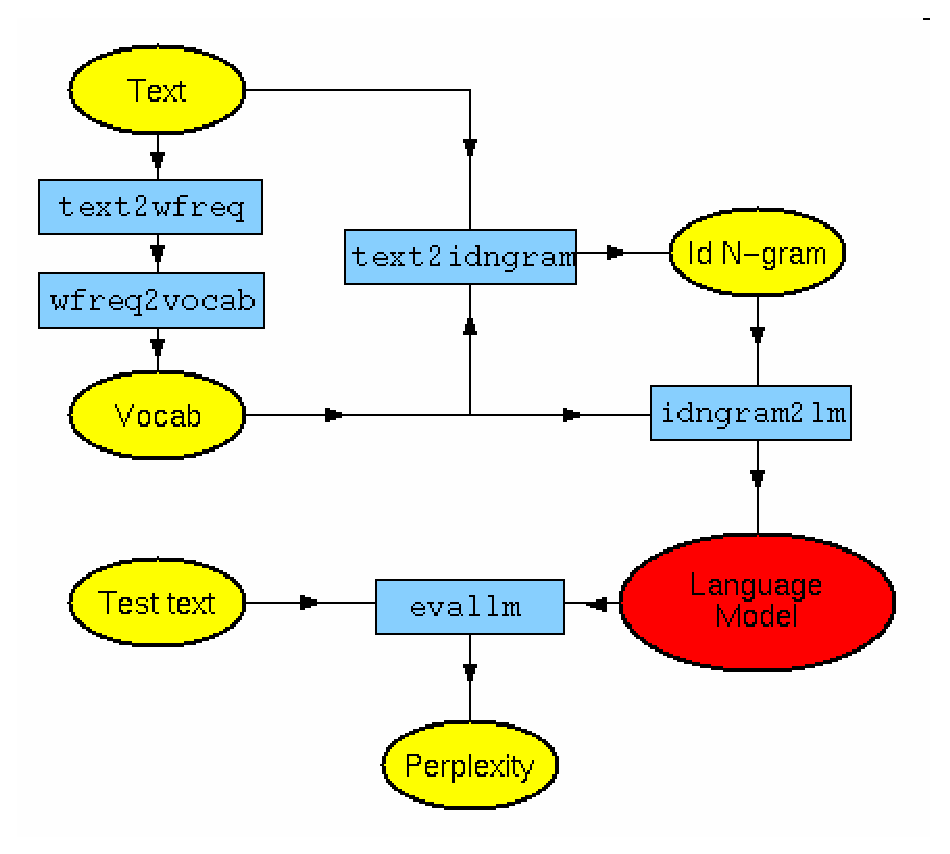
\includegraphics[width=0.5\textwidth]{bilder/toolkit.eps}
	 \caption{Flussdiagramm der typische Anwendung}
  \label{fig:figure_2}
\end{figure}
Der Trainingskorpus und der Testkorpus m\"ussen sorgf\"altig entworfen werden. \cite{book_speech} deutet uns einige Regeln an, dass Trainingskorpora nicht zu spezifisch f\"ur die Aufgabe und auch nicht zu allgemein sein sollen.  
\\
\\
In unseren Experimenten verwenden wir die WSJ (Wall Street Journal) Sprachdatenbank und wir erhalten die Testergebnisse von unterschiedlichen Discounting und M-Gramm-Modellen. In den Experimenten werden am Ende die Parameter \emph{backoff\_from\_un-k\_inc} und \emph{backoff\_from\_unk\_exc} beim Entropieberechnen eingesetzt. Den Unterschied zwischen beiden Parametern findet man in \cite{int_slm_toolkit}.
\\
\\  
Aber es wurde auch eine Problem gefunden, dass beim Absolute-Discounting man nur NAN bekommen kann, wenn man mit komplette wsj-Databasis arbeitet, weil die Vokabulargr\"o\ss e auf 65535 beschr\"anket wird. In der Tabelle 3.1 wird nur die verringerte Trainingbasis (Trainingdaten aus Verzeichnis 88 und Testdaten "`pp\_et\_05.nvp"') angegeben. Die Testdatei "`pp\_et\_05.nvp"' ist von der Trainingbasis unabh"angig.
%table
%table 3.1
\begin{table}[h]
  \begin{center}
  \small\addtolength{\tabcolsep}{-5pt}
    \begin{tabular}{l|l|r|r|r|r|r|r}
     \toprule
     m- &Backoff &\multicolumn{2}{|l|}{Absolute}&\multicolumn{2}{|l|}{Witten-bell}&\multicolumn{2}{l}{Good-Turing}\\
	  \cline{3-8}
	  Gram&(inc/exc)&Perplexit\"at&Entropie&Perplexit\"at&Entropie&Perplexit\"at&Entropie\\
    \hline
    \hline
		Trigramm &inc 	& $292.23$ 	& $8.19$ 	& $291.88$ 	& $8.19$ 	& $307.33$ 	& $8.26$\\
				 		 &exc		& $265.46$ 	& $8.05$ 	& $265.32$ 	& $8.05$ 	& $273.97$ 	& $8.1$\\
		\hline
		Bigramm  &inc 	& $354.2$ 	& $8.47$ 	& $353.4$ 	& $8.47$ 	& $359.32$ 	& $8.49$\\
				 		 &exc		& $330.24$ 	& $8.37$ 	& $329.74$ 	& $8.37$ 	& $334.73$ 	& $8.39$\\
		\hline
		Unigramm &inc 	& $1130.39$ & $10.14$ & $1130.39$ & $10.14$ & $1130.39$ & $10.14$\\
				 		 &exc		& $1130.39$ & $10.14$ & $1130.39$ & $10.14$ & $1130.39$ & $10.14$\\
     \bottomrule
    \end{tabular}
  \end{center}
     \caption{Die Entropie und Perplexit\"at aller Discountings und unterschiedlichen M-Gramme}
\label{tab:table_3}
\end{table}
\\
\\
Aus obigen Testergebnissen kann man als Fazit festhalten, dass Trigramme besser als Bigramme sowie Unigramme sind, \emph{backoff\_from\_unk\_exc} auch besser als \emph{backoff\_from\_u-nk\_inc} . 
		   
\chapter{Automatisierung der Ausf\"uhrung}
\label{chapter:auto_ausfuehrung}
%auto_ausfuehrung

Um das Toolkit automatisch auszuf\"uhren, wurde ein Perl-Script Programm entwickelt. Die Aufgabe des Trainings kann in die folgenden  3 Schritte eingeteilt werden.
\begin{itemize}
	\item Entpackung der Trainingskorpora
	\item Umstellung der Trainingskorpora
	\item Ausf\"uhrung des Toolkits
\end{itemize}
Dazu enth\"alt dieses Programme folgende f\"unf Dateien "`unpack.pl"', "`convertfile.pl"', "`call\_toolkitEx.pl"', "`Pfileoperation.pm"',  "`call\_toolkit.ini"'.\\
Die Datei "`unpack.pl"' hat die Aufgabe, die originale, im Format "`.z"' komprimierte  wsj Dateien zu extrahieren.\\
Die Datei "`convertfile.pl"': tauscht die ung\"ultigen Kuse (<pxxx></p><sxxx></s>) durch g\"ultigen Kuse (<s></s>) aus und ver\"andert alle Buchstaben in Kleine. \\
Die Datei "`call\_toolkitEx.pl"' ist das Hauptprogramm, das SLM-Toolkit aufzurufen.\\ 
Die Datei "`Pfileoperation.pm"' ist ein Perl-Modul\cite{book_perl} als gemeinsame Operationsbibliothek.\\
In der Datei "`call\_toolkit.ini"'  wird die Parameterkonfiguration dargestellt. Darin enthalten sind alle ben\"otigten Parameter wie die Pfade des Toolkits, der Trainingskorpoa, Testkorpus. Ebenso sind die Testparameter wie M-Gramm-Typ und Discounting-Typ auch in dieser Datei definiert. Au\ss erdem wird das \glqq \# \grqq  als Kommentarzeichen verwendet. \"Anderungen an dieser Konfigurationsdatei werden als unterschiedliche Versuche ausgef\"uhrt. Folgend ist ein Beispielkonfiguration angegeben:

\begin{lstlisting}
#notice: only the first value valid.
#==========================================================
#configuration for unpack und converfile
#unpack
#path of .z file 
zsource_path=..//data//source
#specificy unpack path
unpack_path=..//data//target
#converfile
#the output file information. the final file fullname will be
#$convertfile_path//output//$convertfile_name
convertfile_path=..//data//target
convertfile_name=output.text

#==========================================================
# configuration for call_toolkitEx
#SLM pfad
programsource=..//CMU/bin

#trainingcorpus fullpath
filename=...//data/target//output/output.text
#filename=..//data/target//output/output_872.text
#filename=..//data/target//output/output_88.text
#filename=..//data/target//output/output_89.text
#filename=..//data/target//output/output_full.text

#working path
filepath=..//data/target//output/

#cuse file
fileCcs=.//other//lm.ccs

#testcorpus
fileTestText=..//data//test//pp_et_05.nvp

#SLM toolkit running  parameter
#ngram=1
#ngram=2
ngram=3
#discounting=absolute
discounting=good_turing
#discounting=witten_bell
#discounting=linear
#=========================================================

\end{lstlisting}



\chapter{Zusammenfassung}
\label{chapter:zusammenfassung}
%zusammenfassung
Aus unserer Beschreiung bezeichnet sich ein statischer Sprachmodell mit einen approximativen Modell von M-Gramm. Darin werden unterschiedliche Gl\"attungsverfahren eingesetzt, um das Sprachmodell optimiert aufzubauen.
Durch Versuche mit der Sprachmodellrealisierung des SLM-Toolkit ist es bekannt, dass Trigramm besser als Bigramm und Unigramm sind .

Unterschiedliche Kombinationen von Backing-off mit Discounting machen auch einen wichtigen Faktoren.

 
% the chapters
%\chapter{Kurze Einf�hrung}
\label{chapter:introduction}

In diesem Kapitel werden die wichtigsten LaTeX-Konstrukte kurz vorgestellt.\\
Das PDF-Dokument PDF \textit{short-math-guide.pdf} in dem ZIP-Ordner stellt eine gute Anlaufstelle bei Fragen und Problemen (siehe Ordner: \textsc{lesenswertes}).

\section{Formeln}
\label{section:equations}

Dieser Abschnitt befa�t sich mit der Verwendung von Formeln.

\subsection{Inline-Formeln}
\label{subsection:inlineEquation}

Inline-Formeln beginnen und enden mit dem \$-Zeichen: $e^x = \sum\limits_{n=0}^{\infty}\frac{x^n}{n!}$

\subsection{Die equation-Umgebung}
\label{subsection:defaultEquation}

Die im vorherigen Abschnitt \ref{subsection:inlineEquation} eingef�hrte Formel schreibt sich mit Hilfe der \textit{equation}-Umgebung wie folgt:
\begin{equation}
\label{equation:expFunktion}
 e^x = \sum\limits_{n=0}^{\infty}\frac{x^n}{n!}
\end{equation}
Die Exponential-Funktion aus Gleichung \eqref{equation:expFunktion} wird in der Mustererkennung h�ufig verwendet.
ACHTUNG: \textit{eqref} fa�t die Nummer der Gleichung automatisch in runde Klammern.

\section{Literaturquellen referenzieren}
\label{section:literaturref}

Die Literaturquellen werden mit Hilfe von \textsc{bibtex} referenziert. Die Quellen k�nnen in unterschiedlichen  ''.bib'' Dateien beschrieben sein (siehe z.B. \url{bibs/RefA}). Der Aufruf im Dokument erfolgt dann gem��:\\
\textbackslash bibliographystyle\{IEEEtran\}\\
\textbackslash bibliography\{IEEEfull,bibs/RefA, bibs/RefB\}\\
Eine Auflistung aller bibliographystyles findet man z.B. unter \url{http://www.cs.stir.ac.uk/~kjt/software/latex/showbst.html}. Hier wurde der \textit{IEEEtrans} style verwendet, der in der \url{bibs/IEEEtran.bst} definiert wurde. Die Abk�rzungen stehen in \url{bibs/IEEEfull.bib}, welche vor allen Bibliotheken eingebunden wurde. Alle referenzierten  Quellen werden automatisch in das Literaturverzeichnis eingf�gt, ein Fehler erscheint, wenn der \\cite\{\}-Befehl nicht verwendet wurde.\\
Eine Quelle aus einer Datenbank wird so referenziert: \textbackslash cite\{bibtexkey\}.\\
So ist \cite{Digalakis1993} z.B. aus Datenbank RefA und \cite{Lee2007} z.B. aus Datenbank RefB.

\section{Tabellen}
\label{section:tabular}

Dieser Abschnitt befa�t sich mit der Verwendung von Tabellen und den neuen Befehlen des \textit{booktabs}-Packets.
\begin{table}[h]
  \begin{center}
    \begin{tabular}{clr}
      \toprule
      \bf laufende & \bf Wert 1 & \bf Wert 2\\
      \bf Nummer  & [Einheit]  & [Einheit] \\
      \midrule
      $1$ &  $1\,000$ & $20$  \\
      $2$ &  $1\,500$ & $40$  \\
      \bottomrule
    \end{tabular}
  \end{center}
\caption{Eine einfache Tabelle}
\label{tab:table_1}
\end{table}

\section{Grafiken}
\label{section:figures}

Dieser Abschnitt stellt kurz das Einf�gen von Grafiken und das Ersetzen von Text innerhalb einer eps-Datei durch LaTeX-eigene Schriften und insbesonder auch Formeln vor. 

Die Verwendung des \textit{lesenswertes}-Packets wird in der \textit{psfrag-guide.pdf} Datei n�her erkl�rt (siehe Ordner: \textsc{usefullreadings}).\\
\\
ACHTUNG: Die Ersetzungen sind erst in der PS/PDF-Datei an der gew�nschten Stelle. In der DVI-Datei sind die Ersetzungen nur aufgelistet.
\begin{figure}[h]
  \begin{center}
    \resizebox{\textwidth}{!}
    {
    \psfrag{Hintergrund}[][c]{Hintergrund}
    \psfrag{Gesicht}[][c]{Gesicht}
    \psfrag{Detektionskaskade}[][ct]{Detektionskaskade}
    \psfrag{Analyse-}[][ct]{Analyse-}
    \psfrag{fenster}[][c]{fenster}
    \psfrag{W}[][cb]{$\mathcal{W}$}
    \psfrag{Stufe1:}[][ct]{Stufe 1:}
    \psfrag{Stufe 2:}[][ct]{Stufe 2:}
    \psfrag{Stufe 3:}[][ct]{Stufe 3:}
    \psfrag{Stufe 4:}[][ct]{Stufe 4:}
    \psfrag{20 Pixel}[][c]{$|\mathcal{W}_1'|$=$20$ Pixel} 
    \psfrag{40 Pixel}[][c]{$|\mathcal{W}_2'|$=$40$ Pixel} 
    \psfrag{160 Pixel}[][c]{$|\mathcal{W}_3'|$=$160$ Pixel} 
    \psfrag{244 Pixel}[][c]{$|\mathcal{W}_4'|$=$244$ Pixel} 
    \psfrag{T1=}[][c]{$T_1=$}
    \psfrag{T2=}[][c]{$T_2=$}
    \psfrag{T3=}[][c]{$T_3=$}
    \psfrag{0.345}[][c]{$0.345$}
    \psfrag{0.375}[][c]{$0.375$}
    \psfrag{0.385}[][c]{$0.385$}
    \psfrag{T4}[][c]{$T_4$}
    \includegraphics{beispiel.eps}
    }
  \end{center}
  \caption{Eine Grafik mit ersetzten Schriften}
  \label{fig:figure_1}
\end{figure} 





% the chapters
%\chapter{Grafiken die 2.}
\label{chapter:grafiken2}

Der Ort, an dem die Grafiken sich befinden, kann bei der Verwendung des \textit{graphicx} Pakets mit Hilfe des Befehls 
\begin{verbatim}
\graphicspath{{bilder/} {bilder/chapter1/} {bilder/chapter2/}}} 
\end{verbatim}
dem LaTeX-Interpreter vor Begin des Dokuments aber auch an jeder beliebigen Stelle im Dokument neu mitgeteilt werden. Dabei ist darauf zu achten, dass die erneute Verwendung des Befehls die vorherigen Werte �berschreibt. Der Pafd kann alternativ dazu aber auch direkt (relativ oder absolut) dem Befehl \slash includegraphics mitgeteilt werden.
\begin{figure}[h]
  \begin{center}
    \resizebox{0.6\textwidth}{!}{
    \includegraphics{word_phones_states_mixdens.eps}
    }
  \end{center}
  \caption{Verwendung des Pfades der durch \slash graphicspath gegeben ist}
  \label{fig:figure_2}
\end{figure} 
\begin{figure}[h]
  \begin{center}
    \resizebox{0.6\textwidth}{!}{
    \includegraphics{bilder/Kapitel_2/word_phones_states_mixdens.eps}
    }
  \end{center}
  \caption{Verwendung des relativen Pfades}
  \label{fig:figure_3}
\end{figure} 






% ... more to come, hopefully!
\clearpage

%%%%%%%%%%%%%%%%%%%%
% this is where the backmatter starts
% \backmatter % toggling this comment results in chapter names with or without capital numbering
% the bibliography
\addcontentsline{toc}{chapter}{Literaturverzeichnis}
% the bibliography shouldn't have a consecutive numbering
\ihead{\leftmark}
\bibliographystyle{bibs/IEEEtran}
\bibliography{bibs/IEEEfull,bibs/RefA,bibs/RefB,bibs/Ref_xby}
\clearpage
% but the appendix could
\ihead{\thechapter~\leftmark}
% the appendix is part of the backmatter, but uses capital numbering by default
\appendix
%\begin{appendix}
\chapter{Inhalts�bersicht der Begleit-DVD}
Alle Zusatzinformationen sind in digitaler Form auf der beiliegenden DVD enthalten. Im Folgenden wird die Verzeichnisstruktur der DVD erl�utert:
\begin{itemize}
\setlength{\itemsep}{0pt}
  \item \textbf{Ordner 1} -- Enth�lt ...
  \begin{itemize}
    \item[$\bullet$] \textbf{Unterordner 1.1} -- Enth�lt ... .
    \item[$\bullet$] \textbf{Unterordner 2.1} -- Enth�lt ... .
    \item[$\bullet$] \textbf{Unterordner 3.1} -- Enth�lt ... .
    \item[$\bullet$] \textbf{Unterordner 4.1} -- Enth�lt ... .
  \end{itemize}
  \item \textbf{Ordner 2} -- ... .
  \item \textbf{Ordner 3} -- ... .
  \item \textbf{Ordner 4} -- ... .
  \item \textbf{Ordner 5} -- ... .
  \item \textbf{Ordner 6} -- Enth�lt ... :
  \begin{itemize}
    \item[$\bullet$] \textbf{Unterordner 6.1} -- Enth�lt ... .
    \item[$\bullet$] \textbf{Unterordner 6.2} -- Enth�lt ... .
  \end{itemize}
  \item \textbf{Ordner 7} -- Enth�lt ... .
\end{itemize}
Der Inhalt der aufgef�hrten Verzeichnisse ist zur besseren �bersicht ggf. in Unterverzeichnisse aufgeteilt.
\end{appendix}


\end{document}


%%%%%%%%%%%%%%%%%%%%
% this is how to configure kile to take advantage
% of the nomenclature package

% configure kile --> quick build:
% LATEX
% BIBTEX
% LATEX
% LATEX
% VIEWDVI

% use iso 8859-1 or iso 8859-15 to write your text!